% Latex template: mahmoud.s.fahmy@students.kasralainy.edu.eg
% For more details: https://www.sharelatex.com/learn/Beamer

%\documentclass{beamer}					% Document class
% Aspect ratio
\documentclass[aspectratio=169]{beamer}

\setbeamertemplate{footline}[text line]{%
  \parbox{\linewidth}{\vspace*{-8pt}Single molecule localization microscopy \hfill\insertshortauthor\hfill\insertpagenumber}}
\setbeamertemplate{navigation symbols}{}

\usepackage[english]{babel}				% Set language
\usepackage[utf8x]{inputenc}			% Set encoding

\mode<presentation>						% Set options
{
  \usetheme{default}					% Set theme
  \usecolortheme{default} 				% Set colors
  \usefonttheme{default}  				% Set font theme
  \setbeamertemplate{caption}[numbered]	% Set caption to be numbered
}

% Uncomment this to have the outline at the beginning of each section highlighted.
%\AtBeginSection[]
%{
%  \begin{frame}{Outline}
%    \tableofcontents[currentsection]
%  \end{frame}
\usepackage{graphicx}					% For including figures
\usepackage{booktabs}					% For table rules
\usepackage{hyperref}	
\usepackage{tikz-network}				% For cross-referencing
\usepackage[absolute,overlay]{textpos}
\usepackage{bm}
\usepackage[font=small,labelfont=bf]{caption}				% For cross-referencing

\title{Single molecule localization microscopy}	% Presentation title
\author{Clayton W. Seitz}								% Presentation author
\date{\today}									% Today's date	

\begin{document}

% Title page
% This page includes the informations defined earlier including title, author/s, affiliation/s and the date
\begin{frame}
  \titlepage
\end{frame}

\begin{frame}[plain]
  \centering
  \Large A (Very) Brief Summary of SMLM
\end{frame}


\begin{frame}{General principle of single molecle localization microscopy (SMLM)}

\begin{figure}
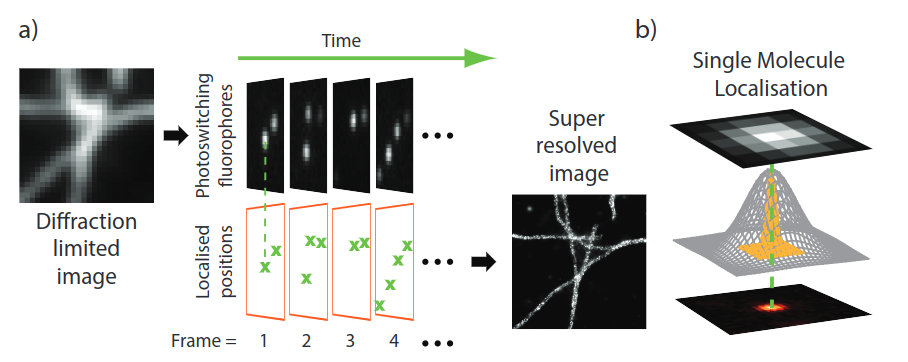
\includegraphics[scale=0.4]{Figure-1}
\end{figure}
\textit{Patel et al. A hidden Markov model approach to characterizing the photo-switching behavior of fluorophores. Annals of Applied Statistics 2019}
\end{frame}

\begin{frame}{SMLM in the time domain}

\begin{figure}
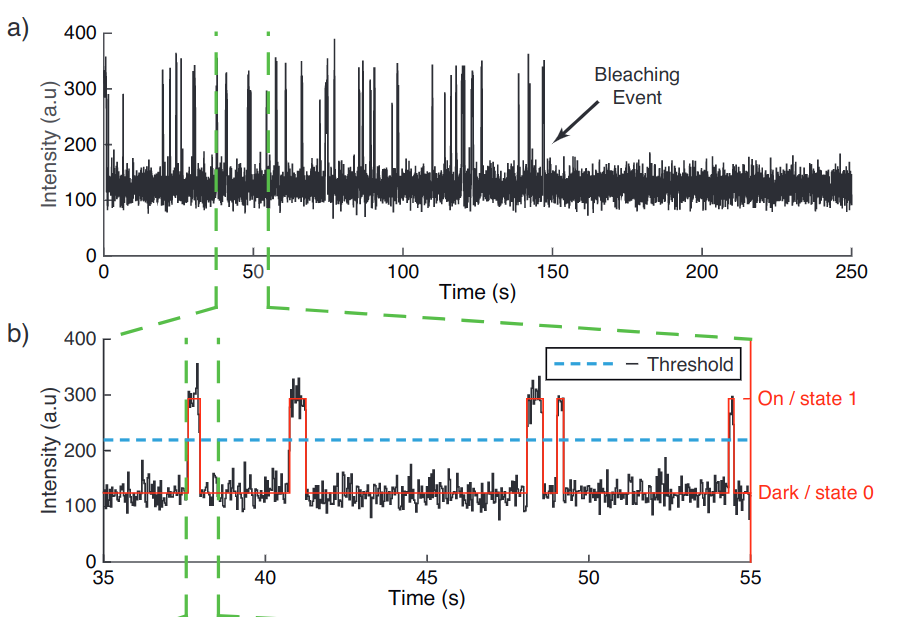
\includegraphics[scale=0.325]{Figure-3}
\end{figure}

\end{frame}

\begin{frame}{Photoswitching is a continuous time Markov process (CTMC)}

\begin{figure}
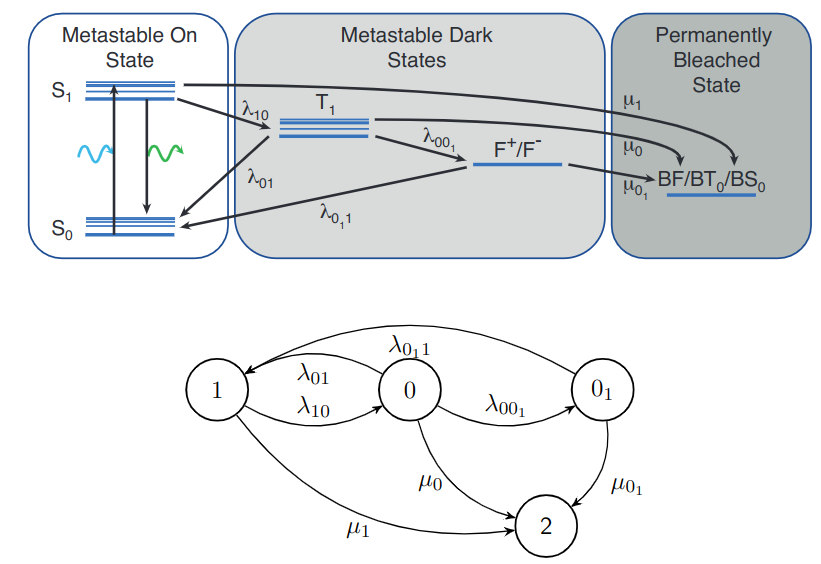
\includegraphics[scale=0.325]{Figure-2}
\end{figure}

\end{frame}

\begin{frame}{The OFF state lifetime depends on laser power (Alexa-647, WFM)}

\begin{figure}
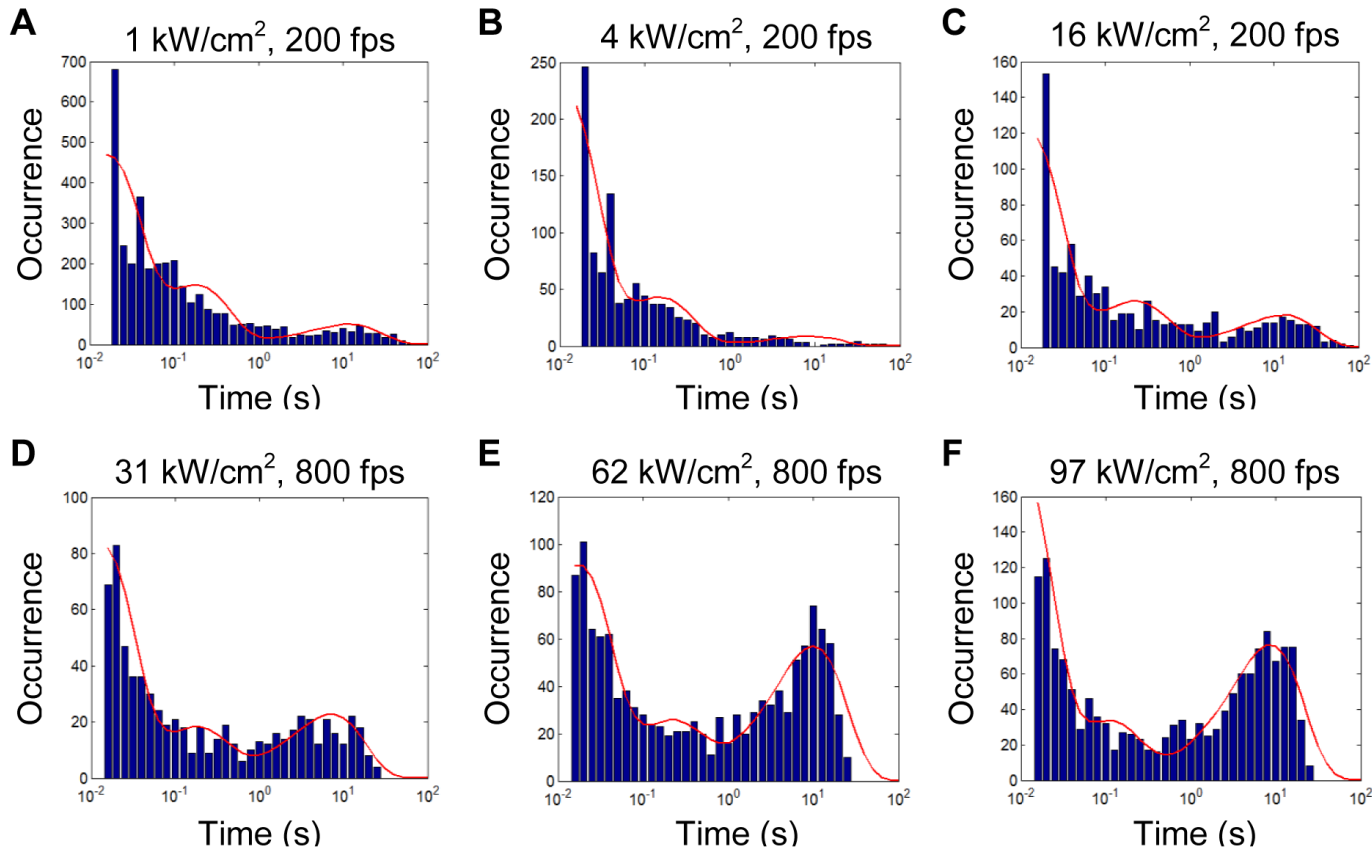
\includegraphics[scale=0.2]{Figure-4}
\end{figure}
\textit{Quantifying and Optimizing Single-Molecule Switching Nanoscopy at High Speeds}
\end{frame}


\begin{frame}{Resolution is dependent on photoswitching kinetics}

\begin{itemize}
\item Define ratio of OFF and ON state lifetimes as $r=\tau_{OFF} /\tau_{ON}$​
\item High values of r assure a low number of fluorophores in the ON state​
\item Low $r$ values ensure precise localization, but acquisitions are slow
\item Long acqusitions are undesirable due to sample drift
\end{itemize}
\vspace{0.2in}
Params for a single molecule are $\theta = (x_{0},y_{0})$
\vspace{0.1in}
What we call lateral ``resolution" in SMLM is the lowest possible uncertainty in $\theta$, given a perfect estimator (The Cramer-Rao lower bound)


\end{frame}

\begin{frame}{Current state of the art for dense localization in 3D (astigmatism)}
DECODE uses a deep generative model to localize dense fluorophores
\begin{figure}
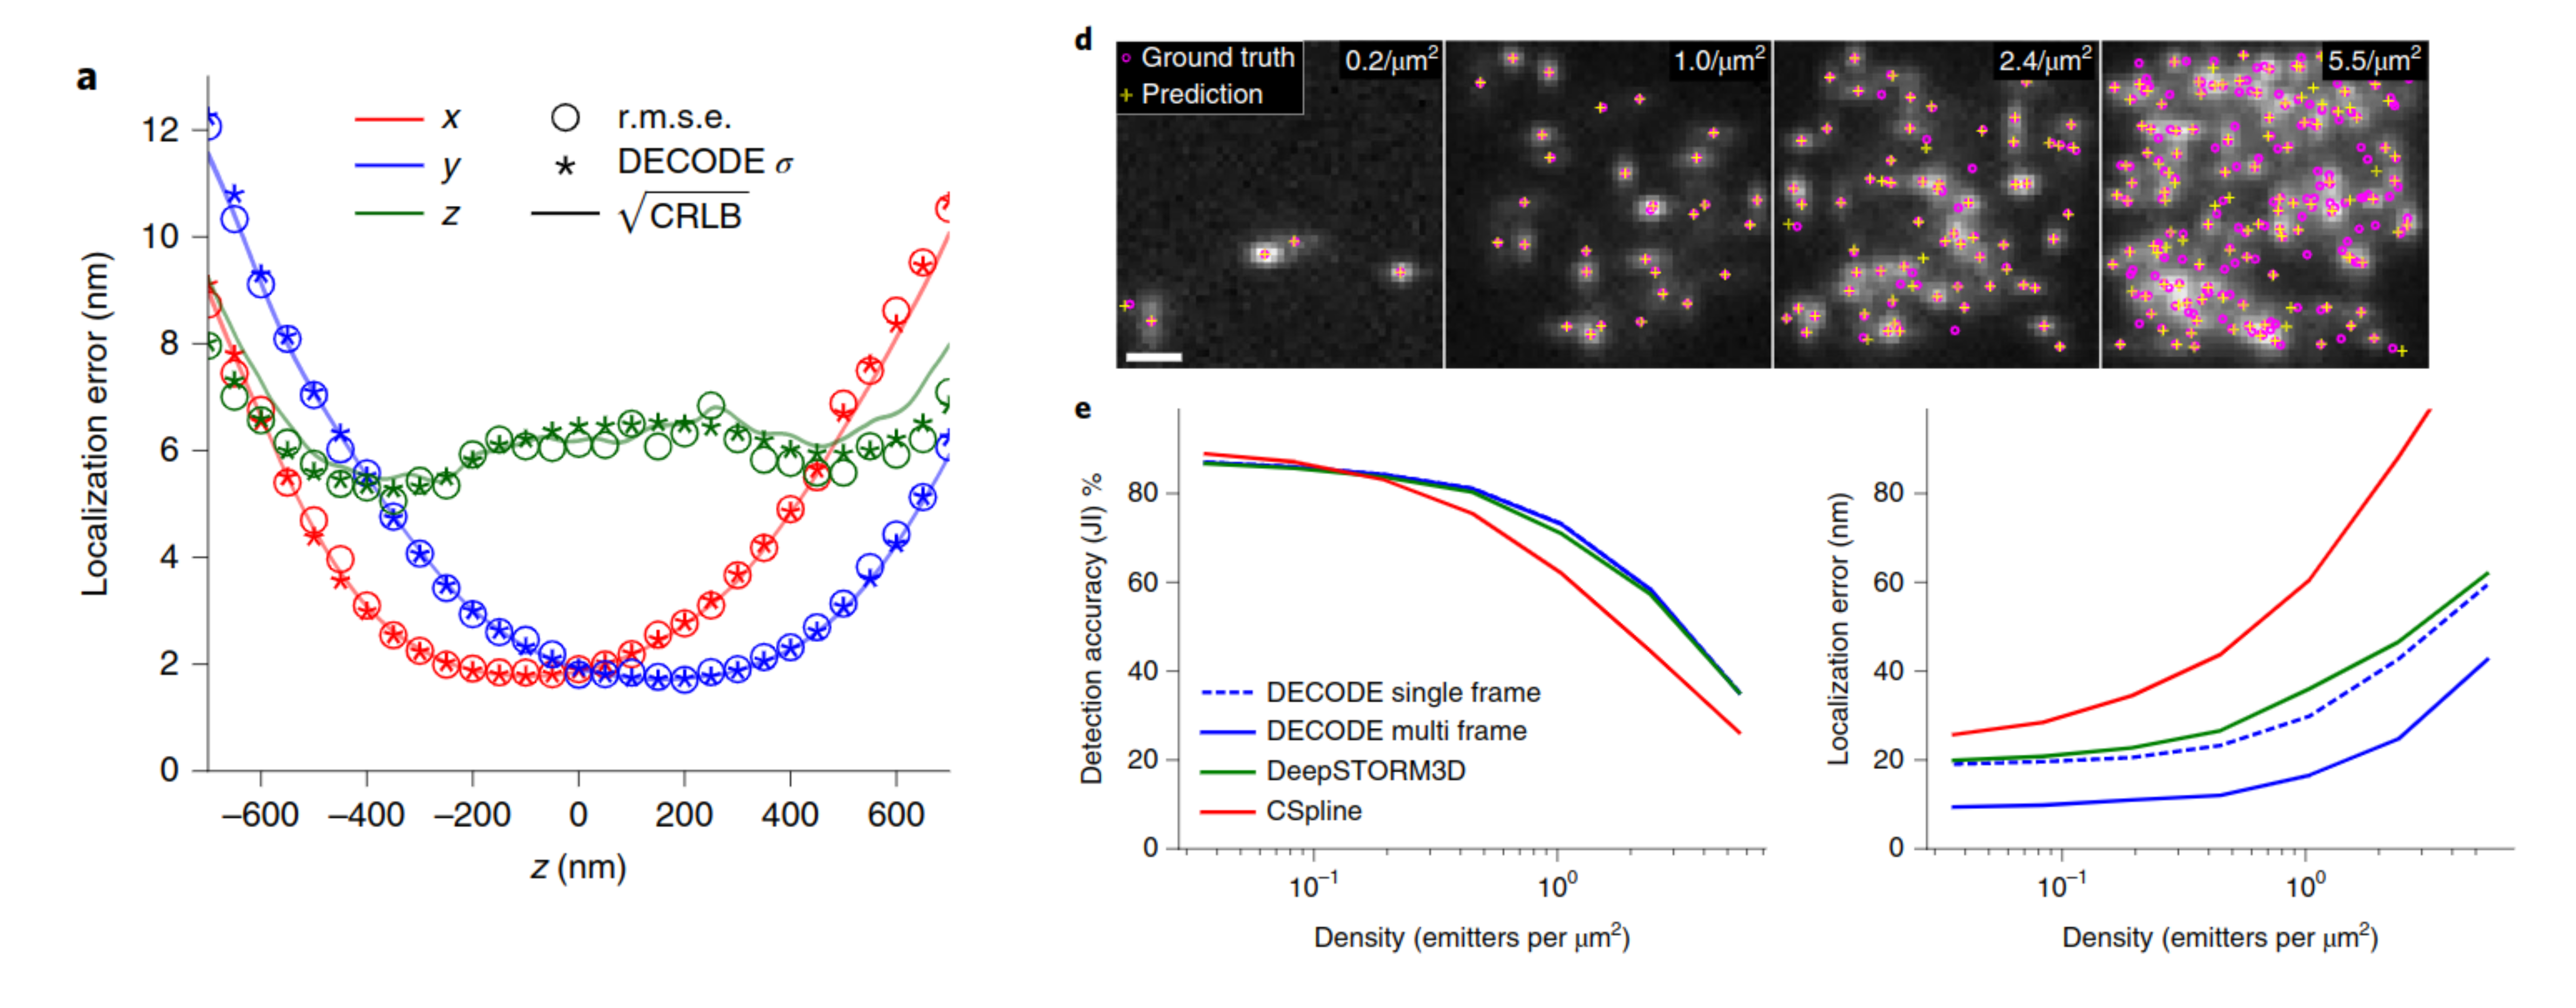
\includegraphics[scale=0.33]{Figure-8}
\end{figure}
\textit{Deep learning enables fast and dense single-molecule localization with high accuracy}
\end{frame}



\begin{frame}[plain]
  \centering
  \Large Mathematical Details
\end{frame}




\begin{frame}{sCMOS noise model}

The Poisson rate parameter for a single pixel is 
\begin{equation*}
\mu_{k} = \eta\Delta t(N_{0}\lambda_{k} + B_{0}) 
\end{equation*}
where $\Delta t$ is the camera exposure time and $N_{0}$ and $B_{0}$ are the fluorophore and background emission rates respectively. 
\begin{equation*}
\lambda_{k} = \int_{\mathrm{pixel}}G(x,y)dxdy
\end{equation*}
where the 2D function $G(x,y)$ is a normalized Gaussian density over the pixel array
\begin{equation*}
\mathrm{G}(x,y) = \frac{1}{2\pi\sigma^{2}}e^{-\frac{(x-x_{0})^{2}+(y-y_{0})^{2}}{2\sigma^{2}}}
\end{equation*}
\end{frame}

\begin{frame}{How to compute $\lambda_{k}$ at each pixel}

We can replace this integral with error functions:

\begin{align*}
\lambda_{x}(x) &= \frac{1}{2}\left(\mathrm{erf}\left(\frac{x+a/2-x_{0}}{\sqrt{2}\sigma}\right) -\mathrm{erf}\left(\frac{x-a/2-x_{0}}{\sqrt{2}\sigma}\right)\right)\\
\lambda_{y}(y) &= \frac{1}{2}\left(\mathrm{erf}\left(\frac{y+a/2-y_{0}}{\sqrt{2}\sigma}\right) -\mathrm{erf}\left(\frac{y-y/2-y_{0}}{\sqrt{2}\sigma}\right)\right)
\end{align*}
For multiple emitters
\begin{equation*}
\lambda(x,y) = \sum_{n}\lambda_{n,x}(x)\lambda_{n,y}(y)
\end{equation*}
The \emph{true signal} is then
\begin{equation*}
\vec{S} = \left[\mathrm{Poisson}(\lambda_{1}), \mathrm{Poisson}(\lambda_{2}), ..., \mathrm{Poisson}(\lambda_{N})\right]
\end{equation*}

\end{frame}

\begin{frame}{Poisson approximation of pixel values}

However, due to readout noise, we measure

\begin{equation*}
\vec{H} = \vec{S} + \vec{\xi}
\end{equation*}
The distribution of $H_{k}$ is the convolution:
\begin{align*}
P(H_{k}|\theta) &= P(S_{k})\circledast P(\xi_{k})\\
&= A\sum_{q=0}^{\infty} \frac{1}{q!}e^{-\mu_{k}}\mu_{k}^{q}\frac{1}{\sqrt{2\pi}\sigma_{k}}e^{-\frac{(H_{k}-g_{k}q-o_{k})}{2\sigma_{k}^{2}}}
\end{align*}
where $P(\xi_{k}) = \mathcal{N}(o_{k},\sigma_{k}^{2})$ and $P(S_{k}) = \mathrm{Poisson}(g_{k}\mu_{k})$. In practice, this expression is difficult to work with, so we look for an approximation. Notice that 

\begin{align*}
\xi_{k} - o_{k} + \sigma_{k}^{2} \sim \mathcal{N}(\sigma_{k}^{2},\sigma_{k}^{2}) \approx \mathrm{Poisson}(\sigma_{k}^{2})
\end{align*}

\end{frame}

\begin{frame}{The model log likelihood and Hessian matrix}
Since $H_{k} = S_{k} + \xi_{k}$, we transform $H_{k}' = H_{k} - o_{k} + \sigma_{k}^{2}$, which is distributed according to 

\begin{align*}
H_{k}' \sim \mathrm{Poisson}(\mu_{k}')\;\;\;\mu_{k}' = g_{k}\mu_{k} + \sigma_{k}^{2}
\end{align*}
Since each Poisson r.v. is independent, the negative log likelihood reads
\begin{align*}
\ell(\vec{H}) &= -\log \prod_{k} \frac{e^{-\left(\mu_{k}'\right)}\left(\mu_{k}'\right)^{n_{k}}}{n_{k}!}\\
&= \sum_{k}  \log n_{k}! + \mu_{k}' - n_{k}\log\left(\mu_{k}'\right)
\end{align*}

\end{frame}

\begin{frame}{The model log likelihood and Hessian matrix}

Fortunately, we can compute the Hessian of the negative log likelihood using the chain-rule for Hessian matrices.

\begin{align*}
\hat{H}_{(\ell,\theta)} = \hat{J}_{(\lambda,\theta)}^{T} \hat{H}_{(\ell,\lambda)} \hat{J}_{(\lambda,\theta)} + (J_{(\ell,\lambda)}\otimes I_{n})\hat{H}_{(\lambda,\theta)}
\end{align*}
By calculating $\hat{H}_{(l,\theta)}$ at $\theta_{\mathrm{MLE}}$, we can get an estimate of the observed information matrix. To do that $J_{(\lambda,\theta)}$ and $H_{(\lambda,\theta)}$ are best left to symbolic calculators. 
\end{frame}


\end{document}